\subsection{Klassische Softwarekomponenten}
\label{sec:2_Softwarekomponente_Klassisch}
\begin{quote}
\glqq The characteristic properties of a component are that it:
\begin{itemize}
\item is a unit of independent deployment
\item is a unit of third-party composition
\item has no (externally) observable state\grqq
\end{itemize}
\end{quote}

Dies ist die Definition einer Komponente von Clemens Szyperski im Buch \glqq Component software: Beyond object-oriented programming\grqq \citereset \autocite{Szyperski.2002}.
Diese Definition bedarf weiterer Erläuterung:
\begin{description}
\item[A component is a unit of independent deployment] \hfill \\
Dieser Punkt der Definition besitzt eine softwaretechnische Implikation. Damit eine Komponente \glqq independent deployable\grqq\ also unabhängig auslieferbar ist, muss sie auch so konzipiert beziehungsweise entwickelt werden. Sämtliche Funktionen der Komponente müssen vollständig unabhängig von der Verwendungsumgebung und von anderen Komponenten sein. Des Weiteren muss der Begriff \glqq independent deployable\grqq\ als Ganzes betrachtet werden, denn es bedeutet, dass eine Komponente nicht partiell, sondern nur als Ganzes ausgeliefert wird. Ein Beispiel für diesen Kontext wäre, dass ein Dritter keinen Zugriff auf die involvierten Komponenten einer Software hat.\\
\item[A component is a unit of third-party composition] \hfill \\
Hier wird der Begriff \glqq composable\grqq\ dahingehend verstanden, dass Komponenten zusammensetzbar sein sollen. In diesem Kontext bedeutet dies, dass eine Applikation aus mehreren Komponenten bestehen kann. Des Weiteren soll auch mit einer Komponente interagiert werden können, was einer klar definierten Schnittstelle bedarf. Nur mit Hilfe dieser Schnittstelle kann garantiert werden, dass die Komponente einerseits vollständig gekapselt von anderen Komponenten ist und andererseits mit der Umgebung interagieren kann. Dies erfordert demnach eine klare Spezifikation, was die Komponente erfordert und was sie bietet.
\item[A component has no (externally observable) state] \hfill \\
Eine Komponente sollte keinen (externen) \glqq observable\grqq also feststellbaren Zustand haben. Die Originalkomponente darf nicht von Kopien ihrer selbst unterschiedlich sein. Wenn Komponenten einen feststellbaren Zustand haben dürften, wäre es nicht möglich, zwei \glqq gleiche\grqq\ Komponenten mit den gleichen Eigenschaften zu haben. Eine mögliche Ausnahme von dieser Regel sind Attribute, die nicht zur Funktionalität der Komponente beitragen. Ein Beispiel in diesem Kontext wäre die Seriennummer für die Buchhaltung. Dieser spezifische Ausschluss ermöglicht einen zulässigen technischen Einsatz eines Zustands, der kritisch für die Leistung sein könnte. Beispielsweise dafür sei der Cache. Eine Komponente kann einen Zustand mit der Absicht zu cachen verwenden. \todo{umschreiben!}Ein Cache ist ein Speicher, auf den man ohne Konsequenzen verzichten kann, jedoch möglicherweise reduzierte Leistung in Anspruch nimmt.
\end{description}

Wenn man eine Komponente mit Hilfe dieser Definition umsetzt, gilt sie als vollständig wiederverwertbar. Des Weiteren ergeben sich aus dieser Definition zwei Sichtweisen auf Komponenten, zum einen die Sichtweise des Verwenders der Komponente (siehe Unterabbildung \ref{sfig:Komponente_Verwender}) und zum anderen die Sichtweise des Entwicklers der Komponente (siehe Unterabbildung \ref{sfig:Komponente_Entwickler}). Der Verwender der Komponente kann keine Aussagen darüber treffen, auf welcher Basis die die verwendete Komponente entwickelt wurde. Folglich kann die Implementierung als \glqq Black-Box\grqq\ für den Verwender gesehen werden. Der Entwickler hingegen hat vollständiges Wissen über den Aufbau und das Verhalten der Komponente.

\begin{figure}[h]
  \centering
  \subfloat[Software-Komponente aus der Sichtweise des Verwenders]{
    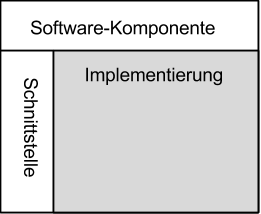
\includegraphics[height=5.0cm]{images/Software-Komponente-Verwender.png}
    \label{sfig:Komponente_Verwender}
  }
  \qquad
  \subfloat[Software-Komponente aus der Sichtweise des Entwicklers]{
    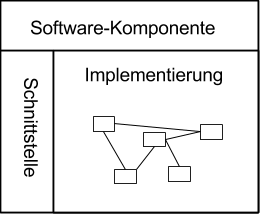
\includegraphics[height=5.0cm]{images/Software-Komponente-Entwickler.png}
    %for reference of this subfigure only
    \label{sfig:Komponente_Entwickler}
  }
  \caption[
    Software-Komponente aus unterschiedlichen Sichtweisen
  ]{
    Software-Komponente aus unterschiedlichen Sichtweisen
  }
  \label{fig:Komponente_Sichtweise}
\end{figure}

In vielen aktuellen Ansätzen sind Komponenten eine schwerwiegende Einheit mit genau einer Instanz in einem System. Beispielsweise könnte ein Datenbankserver eine Komponente darstellen. Oftmals wird der Datenbankserver im Zusammenhang mit der Datenbank als Modul mit einem feststellbaren Zustand angesehen. Dahingehend ist der Datenbankserver ein Beispiel für eine Komponente und die Datenbank ein Beispiel für das Objekt, das von der Komponente verwaltet wird. Es ist wichtig zwischen dem Komponentenkonzept und dem Objektkonzept zu differenzieren, da das Komponentenkonzept in keinster weise den Gebrauch von Zuständen von Objekten fördert beziehungsweise zurückstuft \citereset \autocite{Szyperski.2002}.

Eine Softwarearchitektur ist die zentrale Grundlage einer skalierbaren Softwaretechnologie und ist für komponentenbasierte Systeme von größter Bedeutung. Nur da, wo eine Gesamtarchitektur mit Wartbarkeit definiert ist, finden Komponenten die Grundlage, die sie benötigen. Folgend werden einige Eckpfeiler einer Komponentenarchitektur genannt \citereset \autocite{Szyperski.2002}:
\begin{itemize}
\item Interaktionen zwischen Komponenten und deren Umfeld sind geregelt
\item Die Rollen von Komponenten sind definiert
\item Schnittstellen von Komponenten sind standardisiert
\item Aspekte der Benutzeroberflächen für Endbenutzer und Assembler sind geregelt
\end{itemize}
In Kapitel \ref{sec:2_Softwarearchitektur} auf Seite \pageref{sec:2_Softwarearchitektur} wird der Begriff der Softwarearchitektur näher erläutert. Des Weiteren werden in Kapitel \ref{sec:2_Serviceorientierte_Softwarearchitektur} auf Seite \pageref{sec:2_Serviceorientierte_Softwarearchitektur} und Kapitel \ref{sec:2_Komponentenbasierte_Softwarearchitektur} auf Seite \pageref{sec:2_Komponentenbasierte_Softwarearchitektur} zwei Aspekte der Softwarearchitektur hinsichtlich der Entwicklung mit Komponenten erklärt.
